\chapter{Theory of X-ray Diffraction by Matter}\label{diffraction_theory}\noindent

This chapter gives an overview of the most important tools necessary to
understand X-ray diffraction and provides a simple framework for analysing most
CXDI experiments based on the first Born approximation, also known as
"kinematical" or "single-scattering" approximation. This will be of fundamental
importance when we later try to reconstruct the object that gave rise to a given
diffraction pattern, as  it is obviously impossible to do this if we cannot
predict the diffraction pattern that a given object produces.

\section{Diffraction by a free electron}\label{diffraction_physics}

According to classical electromagnetic theory when a plane monochromatic wave of
amplitude $E_0$, frequency $\nu$, propagating along the $z$ axis
(Fig. \ref{coordinate_axis}a), given by
\begin{equation}
E_i(z,t) = E_0 \exp(2 \pi i \nu (t-z/c)) \, ,
\label{Eq:wave_propagation}
\end{equation}
travels through an electron of charge $e$ and mass $m$ located at the origin of a coordinate
system, that electron will oscilate in the direction of the incident electric 
vector driven by
\begin{equation}
a(t) = \frac{e E_i(0,t)}{m}
\label{Eq:electron_acceleration}
\end{equation}
with a frequency equal to the incoming wave. This in turn will make it radiate
an electric field $E_s$, like any accelerating charge. It follows from Maxwell's
equations that the electric field generated by an accelerating electron is given by
\begin{equation}
E( \mathbf r,t) = \frac{e a_{\perp}(t - |\mathbf r|/c)}{4 \pi \epsilon_0 c^2 r}
\label{Eq:scattering_by_accelerating_charge}
\end{equation}
where  $\epsilon_0$ is the permittivity of free space and $a_{\perp}$ is the acceleration projected on a plane normal to $r$, also called the transverse component of the acceleration (Fig. \ref{coordinate_axis}b). 
\begin{figure}[h]
\centering
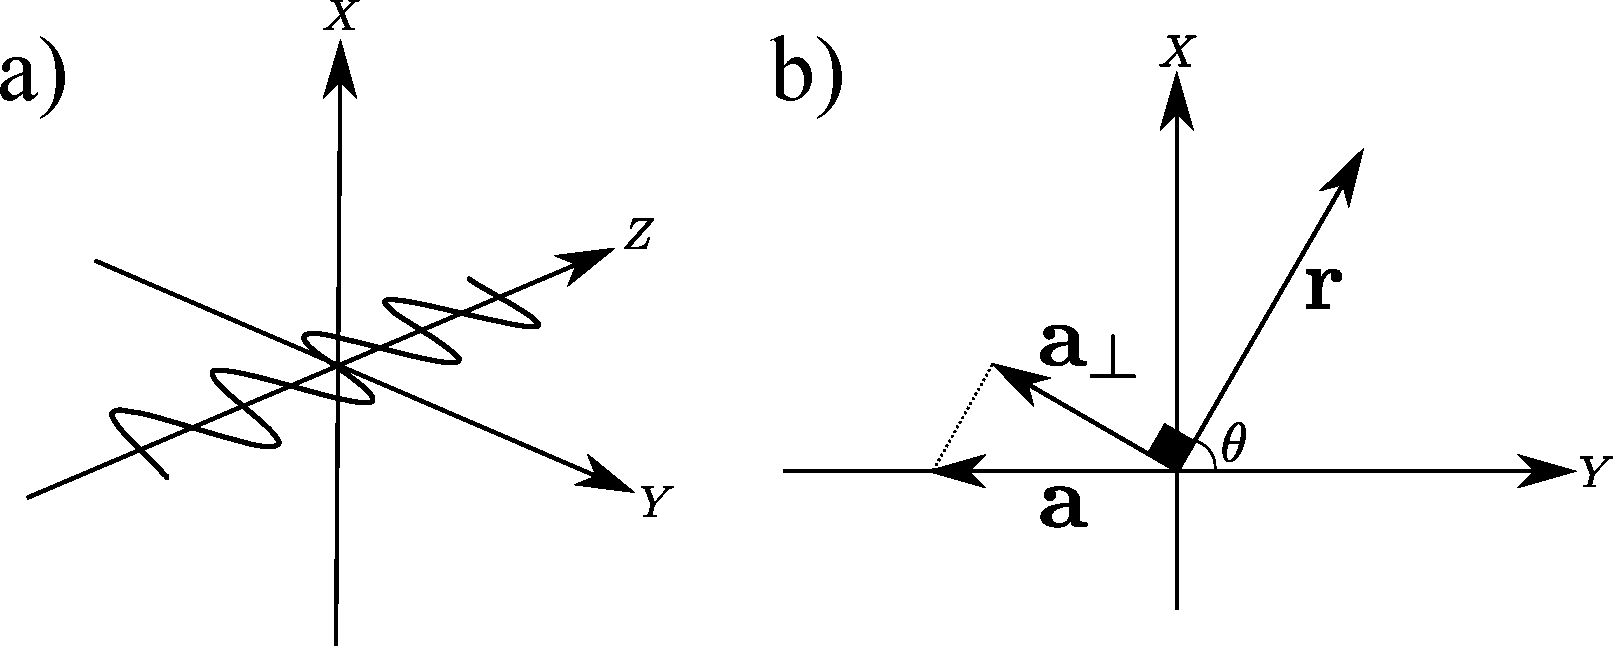
\includegraphics[width=1 \columnwidth]{coordinate_acceleration.pdf}
\caption{a) Monochromatic planar wave linearly polarized along the $y$ axis
  propagating in the positive $z$ direction. b) Transverse component of the
  acceleration sustained by the electron as observed from the position ${\mathbf r}$. $\theta$ is the angle between the polarization axis and the projection of $\mathbf r$ on a plane normal to the propagation direction.}
\label{coordinate_axis}
\end{figure}
Finally combining equations \ref{Eq:wave_propagation},\ref{Eq:electron_acceleration} and \ref{Eq:scattering_by_accelerating_charge} we get that the instantaneous scattered field by a free electron is given by
\begin{eqnarray}
a_{\perp}(t) & = & |\mathbf a(t)| \sin \theta  \\
E(\mathbf r,t) & = & \frac{e^2 E_0 \sin \theta }{4 \pi \epsilon_0 m c^2 r} \exp(2 \pi i \nu (t -| \mathbf r|/c)) 
\label{Eq:scattering_by_electron}
\end{eqnarray}
The classical electron radius is defined as,
\begin{equation}
r_e = \frac{e^2}{4 \pi \epsilon_0 m c^2}
\end{equation}
which can be used to simplify the electric field expression to,
\begin{equation}
E(\mathbf r,t) = \frac{r_e E_0 \sin \theta }{r} \exp(2 \pi i \nu (t -| \mathbf r|/c))  \, .
\end{equation}
The instantaneous scattered power per unit area can then be obtained from the length of the Poynting vector,
\begin{equation} 
S(r,t) = \frac{ E(\mathbf r,t)^2 }{ \epsilon_0 c} .
\label{Eq:poynting_vector}
\end{equation} 
The instantaneous power per unit area scattered by an electron is then,
\begin{equation}
S(r,t)  = \frac{r_e^2 E_0^2 \sin^2 \theta }{\epsilon_0 c r^2} \exp(2 \pi i \nu (t - |\mathbf r|/c)) \, ,
\end{equation}
and the time averaged value is simply,

\begin{equation}
S(r)  = \frac{r_e^2 E_0^2 \sin^2 \theta }{2 \epsilon_0 c r^2}
\end{equation}
The total radiated intensity by a free electron can be calculated by integrating 
have maximum strength on the direction of $E_i$ and zero strength perpedicular
to it
and emit an electric field, $E_s$, described by


using the born-approximation.

- Define Continuous Fourier Transform 

- State some handy properties of the fourier transform like like:

* Symmetry from real functions
* Friedel's law 
* Convolution theorem
* Autocorrelation

- Define DFT

- Talk about sampling and oversampling and define oversampled

- Nyquist frequency

- Aliasing

- Scattering by a free electron

- Scattering by an arbitrary electron density

%%% Local Variables: 
%%% mode: latex
%%% TeX-master: "Thesis"
%%% End: 
